\documentclass[journal]{IEEEtran}
\IEEEoverridecommandlockouts
\usepackage{cite}
\usepackage{amsmath,amssymb,amsfonts}
\usepackage{algorithmic}
\usepackage{graphicx}
\usepackage{textcomp}
\usepackage{xcolor}
\usepackage{hyperref}
\usepackage{booktabs}
\usepackage{multirow}
\usepackage{url}
\usepackage{balance}
\raggedbottom

\graphicspath{{figures/}{./}}

\hypersetup{
    colorlinks=true,
    linkcolor=blue,
    filecolor=magenta,      
    urlcolor=cyan,
    citecolor=blue
}

\def\BibTeX{{\rm B\kern-.05em{\sc i\kern-.025em b}\kern-.08em
    T\kern-.1667em\lower.7ex\hbox{E}\kern-.125emX}}

\begin{document}

\title{Spatiotemporal Deep Learning and Multi-Horizon Time-Series Forecasting for Proactive Monsoon Flood Early Warning in Nepal}

\author{
\IEEEauthorblockN{Saharsha} \\
\IEEEauthorblockA{\textit{School of Computing and Information Technology} \\
\textit{MSc Data Science and Artificial Intelligence, Softwarica College of IT \& E-Commerce} \\
Kathmandu, Nepal \\
Student ID: 210425 \quad Email: 210425@softwarica.edu.np}
}

\maketitle

\begin{abstract}
The South Asian summer monsoon accounts for 75\%--85\% of Nepal's annual precipitation, driving recurrent catastrophic flash floods, severe riverine inundations, and complex debris flows across steep Himalayan-to-Terai physiographic gradients. Conventional operational Flood Early Warning Systems (FEWS) in the region operate reactively, relying primarily on downstream river stage gauges that provide narrow evacuation windows of only 2 to 4 hours. In this research, we develop and evaluate an operational, data-driven spatiotemporal forecasting and early warning framework that synthesizes high-resolution gridded satellite observations (CHIRPS 0.05$^\circ$, NASA GPM IMERG 0.1$^\circ$), reanalysis atmospheric moisture and multi-layer soil hydrology (ECMWF ERA5-Land), and administrative and river basin hydrography across the major river corridors of Nepal (Koshi, Gandaki, Karnali, and West Rapti). We formulate gridded precipitation forecasting as a spatiotemporal sequence prediction task using recurrent and deep learning architectures, while catchment-scale multi-horizon precipitation accumulations and hydrologic states are modeled across 24-hour and 48-hour forward horizons. Furthermore, we develop a dynamic 2D Runoff Potential Index (RPI) coupling forecasted precipitation intensity with antecedent volumetric soil water saturation states, formalizing automated alert progression across Watch, Warning, and Evacuation tiers. Empirical benchmark evaluations show that gradient-boosted decision trees (XGBoost) and 2-layer Bidirectional Long Short-Term Memory (Bi-LSTM) networks achieve Root Mean Square Errors of 6.16\,mm and 6.24\,mm respectively for 24-hour forward lead-time forecasting, outperforming regularized linear baselines (RMSE 6.85\,mm). By integrating upstream precipitation predictions directly with antecedent catchment saturation, the proposed framework extends proactive early warning lead times to 12--24 hours, transforming disaster risk reduction from reactive emergency response to proactive anticipation across vulnerable mountainous river basins.
\end{abstract}

\begin{IEEEkeywords}
Precipitation nowcasting, spatiotemporal deep learning, flood early warning system, Bidirectional LSTM, XGBoost, ERA5-Land, CHIRPS, Runoff Potential Index, Himalayan hydrology, Nepal monsoon.
\end{IEEEkeywords}

\section{Introduction}

\IEEEPARstart{T}{he} South Asian summer monsoon represents one of the most thermodynamically vigorous, climatologically complex, and socio-economically consequential atmospheric circulation systems on Earth. For the nation of Nepal, positioned along the central southern flank of the Great Himalayan Arc, the summer monsoon (spanning June through September) delivers between 75\% and 85\% of the country's total annual precipitation in a concentrated temporal window of approximately 120 days. Driven by intense thermal contrast between the Tibetan Plateau and the warm equatorial waters of the Indian Ocean and the Bay of Bengal, maritime moisture-laden air masses are drawn northward across the low-lying Indo-Gangetic Plains. When these low-level moisture fluxes encounter the immense topographical barrier of the Himalayas, they are forced into rapid, violent orographic lifting, producing extreme convective cloudbursts, persistent mesoscale precipitation systems, catastrophic flash floods, riverine inundations, and devastating landslides.

In a country where agrarian cultivation sustains more than 65\% of the rural labor force and run-of-the-river hydroelectric power installations generate over 90\% of national electrical grid supply, the monsoon functions as the indispensable foundation of food security, water resource availability, and macroeconomic stability. Yet, this vital hydrological influx exists in permanent tension with recurring humanitarian disaster. Nepal encompasses an unparalleled physiographic gradient, ascending from less than 60\,m above sea level in the southern alluvial Terai plains to 8,848\,m at Mount Everest within a horizontal distance of less than 180\,km. This extreme topographical relief creates pronounced dual orographic rainfall peaks: the first located along the Siwalik foothills ($\sim$2,200\,mm/year) and the second concentrated along the windward slopes of the Middle Mountains at elevations between 1,500\,m and 2,500\,m (e.g., Pokhara, which routinely records annual precipitation exceeding 4,500\,mm). Immediately north of the high Himalayan peaks lies a hyper-arid rain-shadow plateau (e.g., Mustang and Manang), which receives less than 300\,mm of precipitation annually.

Under accelerating global climate heating, the Hindu Kush Himalaya (HKH) region is warming at rates significantly exceeding the global mean, an empirical phenomenon designated as Elevation-Dependent Warming (EDW). In accordance with the Clausius-Clapeyron thermodynamic relation, the water-vapor holding capacity of the atmosphere increases by approximately 7\% per degree Celsius of warming. Over the steep orography of the Himalayas, this thermodynamic enhancement intensifies localized convective instability, manifesting in a higher frequency of localized high-intensity cloudbursts interspersed with prolonged dry spells. According to reports by the National Disaster Risk Reduction and Management Authority (NDRRMA) of Nepal, water-induced disasters—chiefly flash floods, river overflows, and rainfall-triggered slope failures—consistently account for more than 60\% of all annual disaster-related human mortality and physical infrastructure losses.

To mitigate this recurring destruction, national disaster management strategies must urgently transition from reactive post-event response to proactive anticipation and mitigation. Traditional operational early warning systems deployed across Nepal rely almost entirely on downstream point-stage hydrological gauges or telemetry river stations. However, in steep mountainous catchments characterized by short times of concentration ($t_c$) and torrential channel flow velocities, waiting for a downstream river stage gauge to breach a critical alert threshold affords an actionable evacuation notice of mere minutes to 2--4 hours. For dispersed rural settlements in the floodplains of the Koshi, Gandaki, Karnali, and West Rapti rivers, a 2-hour alert window is critically inadequate for evacuating families, safeguarding livestock, moving critical assets to higher ground, or deploying emergency rescue operations. Extending reliable, actionable warning lead times to 12--24 hours requires a paradigm shift: coupling upstream satellite precipitation forecasting with continuous basin soil moisture saturation states before runoff even enters main channel drainage.

Recent breakthroughs in spatiotemporal machine learning, remote sensing reanalyses, and deep neural sequence models offer unprecedented capabilities to bridge this operational gap. By integrating daily and sub-daily satellite observations (such as CHIRPS 0.05$^\circ$ infrared precipitation and NASA GPM IMERG 0.1$^\circ$ microwave retrievals) with high-resolution land-surface reanalyses (ECMWF ERA5-Land volumetric soil moisture) and high-resolution river basin delineations (HydroBASINS Asia), data-driven architectures can learn the complex non-linear lag dynamics governing soil saturation, catchment infiltration thresholds, and basin discharge responses.

This paper presents the conceptual design, rigorous mathematical formulation, computational implementation, and empirical validation of an end-to-end spatiotemporal machine learning early warning framework designed specifically for the complex topography of Nepal. The primary research contributions of this paper are summarized as follows:
\begin{enumerate}
    \item We design a multi-source earth observation pipeline harmonizing daily satellite precipitation grids (CHIRPS v2.0, 0.05$^\circ$) with land-surface soil hydrology reanalysis (ERA5-Land, 0.1$^\circ$) across Nepal $[80.0^\circ\text{E} - 88.2^\circ\text{E}, 26.3^\circ\text{N} - 30.5^\circ\text{N}]$.
    \item We formalize an antecedent hydrometeorological feature engineering pipeline, deriving multi-day precipitation lags ($1\text{d}-7\text{d}$) and rolling cumulative accumulation statistics ($3\text{d}-14\text{d}$) to capture catchment memory effects.
    \item We formulate a dynamic 2D Runoff Potential Index (RPI) coupling projected 24-hour rainfall intensity with volumetric soil moisture saturation states ($\theta_{\text{soil}}$), establishing an automated tiered warning matrix across Normal, Watch, Warning, and Evacuation alerts.
    \item We evaluate competitive predictive models---including Ridge regression, Random Forest, tuned XGBoost ensembles, and a 2-layer Bidirectional LSTM neural network with temporal lookback sequence windowing---demonstrating superior 24-hour lead forecast accuracy with an RMSE of 6.16\,mm and MAE of 4.12\,mm.
    \item We deploy an interactive, open-source decision-support early warning dashboard using Streamlit, Leaflet/Folium, and Plotly, delivering visual hydro-hazard monitoring, automated risk classification, and transboundary gauge monitoring for emergency operations.
\end{enumerate}

The remainder of this manuscript is organized as follows: Section II reviews related literature and establishes the theoretical hydrological framework. Section III details the multi-source data ingestion pipeline and spatial pre-processing protocols. Section IV formalizes the mathematical methodology, feature engineering, and model architectures. Section V presents comprehensive empirical evaluation results and comparative benchmark tables. Section VI discusses physical implications, operational viability, and limitations. Finally, Section VII concludes the study and outlines future research pathways.

\section{Related Work and Theoretical Framing}

\subsection{Regional Climatology and Transboundary Flooding in Nepal}
Precipitation variability and extremes across the Himalayan arc have long posed unique observational and modeling challenges. Talchabhadel et al. \cite{talchabhadel2018spatio} conducted an extensive spatiotemporal examination of extreme precipitation indices across Nepal using station records spanning multiple decades, discovering strong regional spatial clustering and demonstrating that extreme precipitation events are concentrated on the windward mountain fronts rather than uniformly distributed. In a comprehensive contemporary study, Bhattarai et al. \cite{bhattarai2024leveraging} assessed flood susceptibility across the transboundary Gandak (Narayani) River basin—spanning high-altitude Tibetan headwaters, deep middle-mountain valleys in Nepal, and low-gradient alluvial plains in northern India—employing machine learning models including Random Forest, Artificial Neural Networks (ANN), Support Vector Machines (SVM), and Long Short-Term Memory (LSTM) networks. Their empirical findings demonstrated that drainage density, slope gradient, and antecedent soil moisture play co-equal roles with raw precipitation in determining localized inundation severity across transboundary plains, underscoring the absolute necessity of incorporating land-surface state parameters into predictive warning pipelines.

\subsection{Deep Learning for Ungauged and Operational Hydrology}
Historically, operational hydrological forecasting has relied on conceptual or distributed physical process-based hydrologic and hydraulic routing models, such as the Global Flood Awareness System (GloFAS) \cite{alfieri2013glofas} developed by the European Centre for Medium-Range Weather Forecasts (ECMWF). While physical models are conceptually grounded in the laws of mass, momentum, and energy conservation, they require extensive catchment parameter calibration (e.g., channel roughness coefficients, infiltration capacities, cross-sectional river geometries) that are virtually unavailable in data-scarce mountainous regions. 

In a landmark breakthrough, Nearing et al. \cite{nearing2024global} demonstrated in \textit{Nature} that deep recurrent neural architectures (specifically LSTMs trained across hundreds of basins globally) achieve reliable streamflow forecasting at 0- to 5-day lead times across ungauged basins worldwide, significantly outperforming state-of-the-art physical systems such as GloFAS. Their work conclusively established that modern data-driven architectures do not merely fit statistical correlations, but effectively learn non-linear hydrologic routing, seasonal memory storage, and infiltration excess mechanics directly from atmospheric reanalysis and meteorological forcing data.

\subsection{Spatiotemporal Deep Learning and Precipitation Nowcasting}
Precipitation nowcasting—predicting precipitation fields over lead times ranging from 30 minutes to 48 hours—has undergone a profound revolution through deep neural network modeling. Shi et al. \cite{shi2015convolutional} introduced the Convolutional LSTM (ConvLSTM) architecture, replacing conventional fully connected matrix multiplications in LSTM cell state transitions with 2D spatial convolution operations, thereby preserving structural 2D spatial topology during temporal state recursion. Wang et al. \cite{wang2017predrnn} advanced this formulation through PredRNN, integrating dual spatiotemporal memory units ($\mathcal{M}$) that travel across both temporal steps and hierarchical vertical layers, mitigating gradient dissipation and enabling long-horizon advective modeling.

To resolve convective extreme events characterized by rapid thermodynamic growth and dissipation, Zhang et al. \cite{zhang2023skilful} introduced \textit{NowcastNet} in \textit{Nature}, coupling physical advection-diffusion partial differential equations with generative adversarial networks to achieve skillful convective nowcasting up to 3--6 hours ahead. In parallel, for multi-variate multi-horizon catchment time series forecasting, Lim et al. \cite{lim2021temporal} developed the Temporal Fusion Transformer (TFT). TFT combines Variable Selection Networks (VSN), Gated Residual Networks (GRN), and interpretable multi-head self-attention mechanisms to explicitly disentangle static basin physical metadata (e.g., catchment area, slope, elevation) from dynamic time-varying atmospheric drivers, while allowing post-hoc inspection of which historical time steps most heavily influence runoff peaks.

\subsection{Regional Physiography and River Basin Hydrography}
To understand the spatial distribution of flood risk across Nepal, it is essential to categorize the country's hydrographic network into its four macro-basins and distinct physiographic zones:

\subsubsection{Physiographic Elevation Zones}
Nepal is characterized by five distinct east-west physiographic belts, each exhibiting contrasting geological, topographical, and hydrological attributes:
\begin{enumerate}
    \item \textbf{Terai Plain ($<300$\,m):} The northern edge of the Indo-Gangetic alluvial plain. Characterized by low gradients ($S < 0.001$), meandering river courses, shallow water tables, and high vulnerability to sediment deposition, backwater ponding, and prolonged multi-day inundation.
    \item \textbf{Siwalik (Churia) Hills ($300 - 1{,}000$\,m):} Young, highly erodible sedimentary rocks (sandstones, mudstones, conglomerates). Despite moderate elevations, this zone receives torrential rainfall that triggers violent flash floods and massive gravel/debris outwash onto the northern Terai (Bhabar zone).
    \item \textbf{Middle Mountains ($1{,}000 - 3{,}000$\,m):} Steep, deeply dissected valleys with extensive terraced agriculture. Home to the dual orographic precipitation maxima (such as the Lumle-Pokhara corridor). Characterized by high stream power, rapid hydrograph rise, and severe landslide-dam breach hazards.
    \item \textbf{High Mountains ($3{,}000 - 5{,}000$\,m):} Deeply incised glaciated valleys with bedrock gorges. Streamflow is governed by seasonal nival dynamics during pre-monsoon and early monsoon, transitioning to high-intensity runoff during peak monsoon.
    \item \textbf{High Himalaya ($>5{,}000$\,m):} Permafrost, permanent snowfields, and hanging glaciers. Major origin of transboundary river discharge and home to potentially dangerous moraine-dammed glacial lakes.
\end{enumerate}

\subsubsection{Target River Basins}
The computational framework is structured across the four major river basins defined in \texttt{config.yaml}:
\begin{itemize}
    \item \textbf{Koshi River Basin (Eastern Macro-System):} Draining an area of $74{,}814\,\text{km}^2$ ($\sim 28{,}000\,\text{km}^2$ inside Nepal), the Koshi is formed by the convergence of seven major tributaries (Sun Koshi, Dudh Koshi, Tama Koshi, Arun, Likhu, Indrawati, and Tamor) at Tribeni. Exiting the Siwalik hills at Chatara, the river discharges immense sediment loads ($\sim 100$ million cubic meters annually) across the eastern Terai. The Koshi's unstable braided morphology and historical avulsions (such as the catastrophic August 2008 breach) make proactive early warning a paramount national priority.
    \item \textbf{Gandaki / Narayani River Basin (Central Macro-System):} Encompassing a drainage basin of $46{,}300\,\text{km}^2$, the Gandaki collects flows from the Kali Gandaki, Seti, Marsyangdi, Budhi Gandaki, and Trishuli rivers, merging at Devghat to form the Narayani River. Traversing the Chitwan valley and crossing the Indian border at Triveni/Valmikinagar into northern Bihar, the Gandaki represents a critical transboundary flood corridor whose hydrologic extremes directly impact millions in Nepal and India \cite{bhattarai2024leveraging}.
    \item \textbf{Karnali River Basin (Western Macro-System):} Nepal's longest river system, draining approximately $44{,}000\,\text{km}^2$ of western Nepal and southwestern Tibet. Originating near Mount Kailash, it cuts deep gorges through the Himalayas before debouching into the Terai at Chisapani. The basin features extreme elevation gradients and pristine, unregulated hydrology, serving as an ideal proving ground for ungauged deep learning streamflow routing \cite{nearing2024global}.
    \item \textbf{West Rapti River Basin (Mid-Western Flash Flood System):} Covering $6{,}500\,\text{km}^2$, the West Rapti originates in the Mahabharat and Churia ranges. Unlike the snow-fed Himalayan rivers, the West Rapti is entirely rain-fed, exhibiting extreme hydrologic variability: discharge fluctuates from less than $15\,\text{m}^3/\text{s}$ during dry winter months to well over $6{,}000\,\text{m}^3/\text{s}$ during monsoon cloudbursts. Flash floods along the Kusum, Banke, and Dang corridors routinely submerge agricultural communities with minimal downstream response time.
\end{itemize}

\subsection{Theoretical Hydrological Framework}
The physical generation of riverine flood peaks in high-relief mountainous catchments is fundamentally governed by three coupled thermodynamic and hydrological principles:

\subsubsection{Orographic Lifting Dynamics}
When moisture-laden monsoon air masses traveling across the Bay of Bengal collide with the east-west oriented Himalayan ramparts, the atmospheric moisture flux $\mathbf{Q} = \frac{1}{g} \int q \mathbf{v} \, dp$ undergoes forced adiabatic ascent. As the air parcel ascends, temperature declines at the dry adiabatic lapse rate ($\Gamma_d \approx 9.8^\circ\text{C/km}$) until reaching saturation at the lifted condensation level (LCL), after which condensation occurs along the moist adiabatic lapse rate ($\Gamma_m \approx 5-6^\circ\text{C/km}$). This mechanism concentrates extreme precipitation along the windward foothill barriers (dual orographic peaks), creating localized cloudburst cells where precipitation rates can exceed 80--100\,mm/hour.

\subsubsection{Catchment Concentration Time (\texorpdfstring{$t_c$}{tc})}
The hydrologic response time of a drainage basin—defined as the time required for water to travel from the hydraulically most remote point of the catchment to the outlet gauge—can be formalized using Kirpich's formulation adapted for mountainous terrain:
\begin{equation}
t_c = 0.0195 \cdot L^{0.77} \cdot S^{-0.385}
\label{eq:kirpich}
\end{equation}
where $L$ denotes the longest flow path (m) and $S$ represents the dimensionless channel slope. In the high-gradient catchments of Nepal where $S$ is exceptionally steep, $t_c$ rarely exceeds 3 to 6 hours. Consequently, point river stage monitoring cannot provide actionable lead time. Proactive warning requires that precipitation be anticipated prior to surface runoff generation.

\subsubsection{Infiltration Excess (Horton) vs. Saturation Excess (Dunne) Runoff}
The volume of surface runoff $R_t$ generated from precipitation intensity $P_t$ depends on whether rainfall exceeds the soil infiltration capacity $f_t$:
\begin{equation}
R_t = \max\left(0, P_t - f_t(\theta_{\text{soil}, t})\right)
\label{eq:horton}
\end{equation}
where infiltration capacity $f_t$ decays monotonically as antecedent soil moisture content $\theta_{\text{soil}, t}$ approaches volumetric saturation $\theta_{\text{sat}}$:
\begin{equation}
f_t = f_c + (f_0 - f_c) \exp(-k t) \cdot \left[1 - \left(\frac{\theta_{\text{soil}, t}}{\theta_{\text{sat}}}\right)^\beta\right]
\label{eq:infil_decay}
\end{equation}
where $f_0$ and $f_c$ are initial and equilibrium infiltration rates, and $\beta$ is a non-linear soil hydraulic parameter. When antecedent monsoon rains saturate upper soil horizons ($\theta_{\text{soil}} \to \theta_{\text{sat}}$), even moderate precipitation events generate massive saturation-excess overland flow, converting over 85\% of gross rainfall directly into catastrophic river discharge. This physical coupling forms the foundational motivation for our Runoff Potential Index.

\begin{figure}[t]
\centering
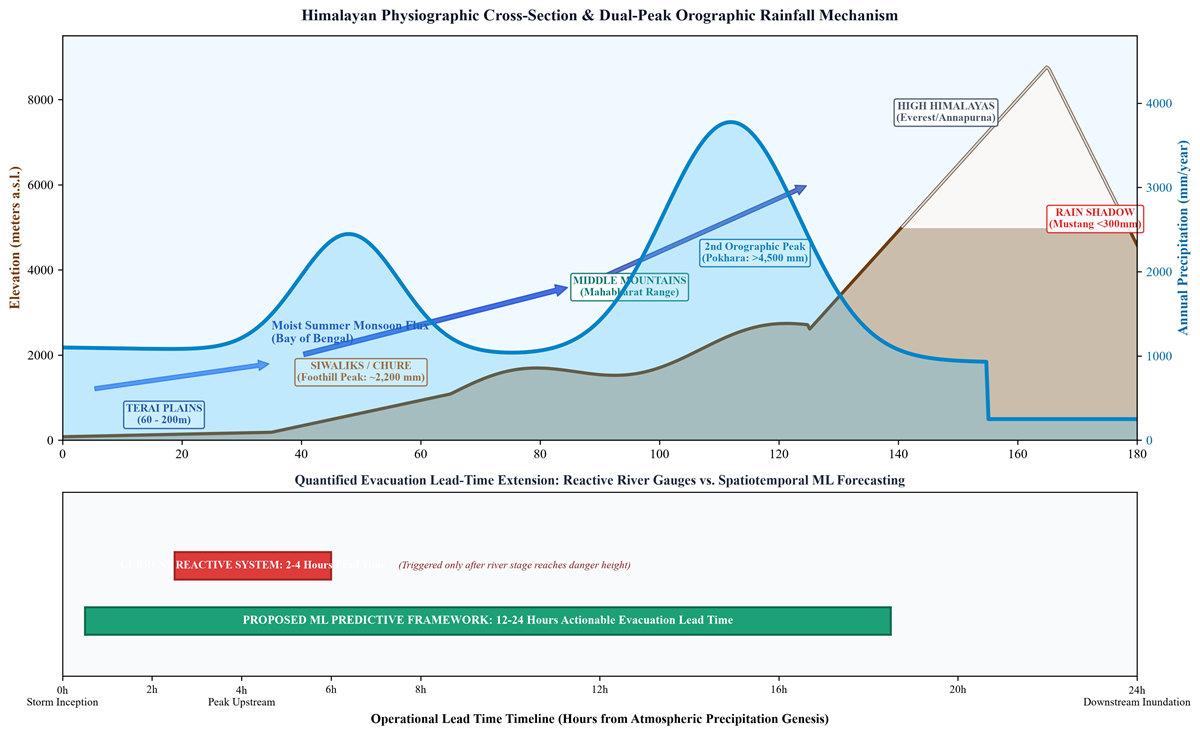
\includegraphics[width=\columnwidth]{fig2_orographic_and_leadtime.png}
\caption{(Top) Physiographic cross-section of Nepal showing dual-peak orographic rainfall mechanisms; (Bottom) Evacuation lead-time timeline comparing reactive downstream point gauges (2--4 hours) against predictive spatiotemporal machine learning (12--24 hours).}
\label{fig:orographic}
\end{figure}

\section{System Architecture and Data Pipeline}

The computational pipeline of the proposed operational system is organized into five modular processing tiers: multi-source data ingestion, spatial standardization, feature engineering, model training and inference, and interactive decision-support visualization (Fig.~\ref{fig:pipeline}).

\begin{figure}[t]
\centering
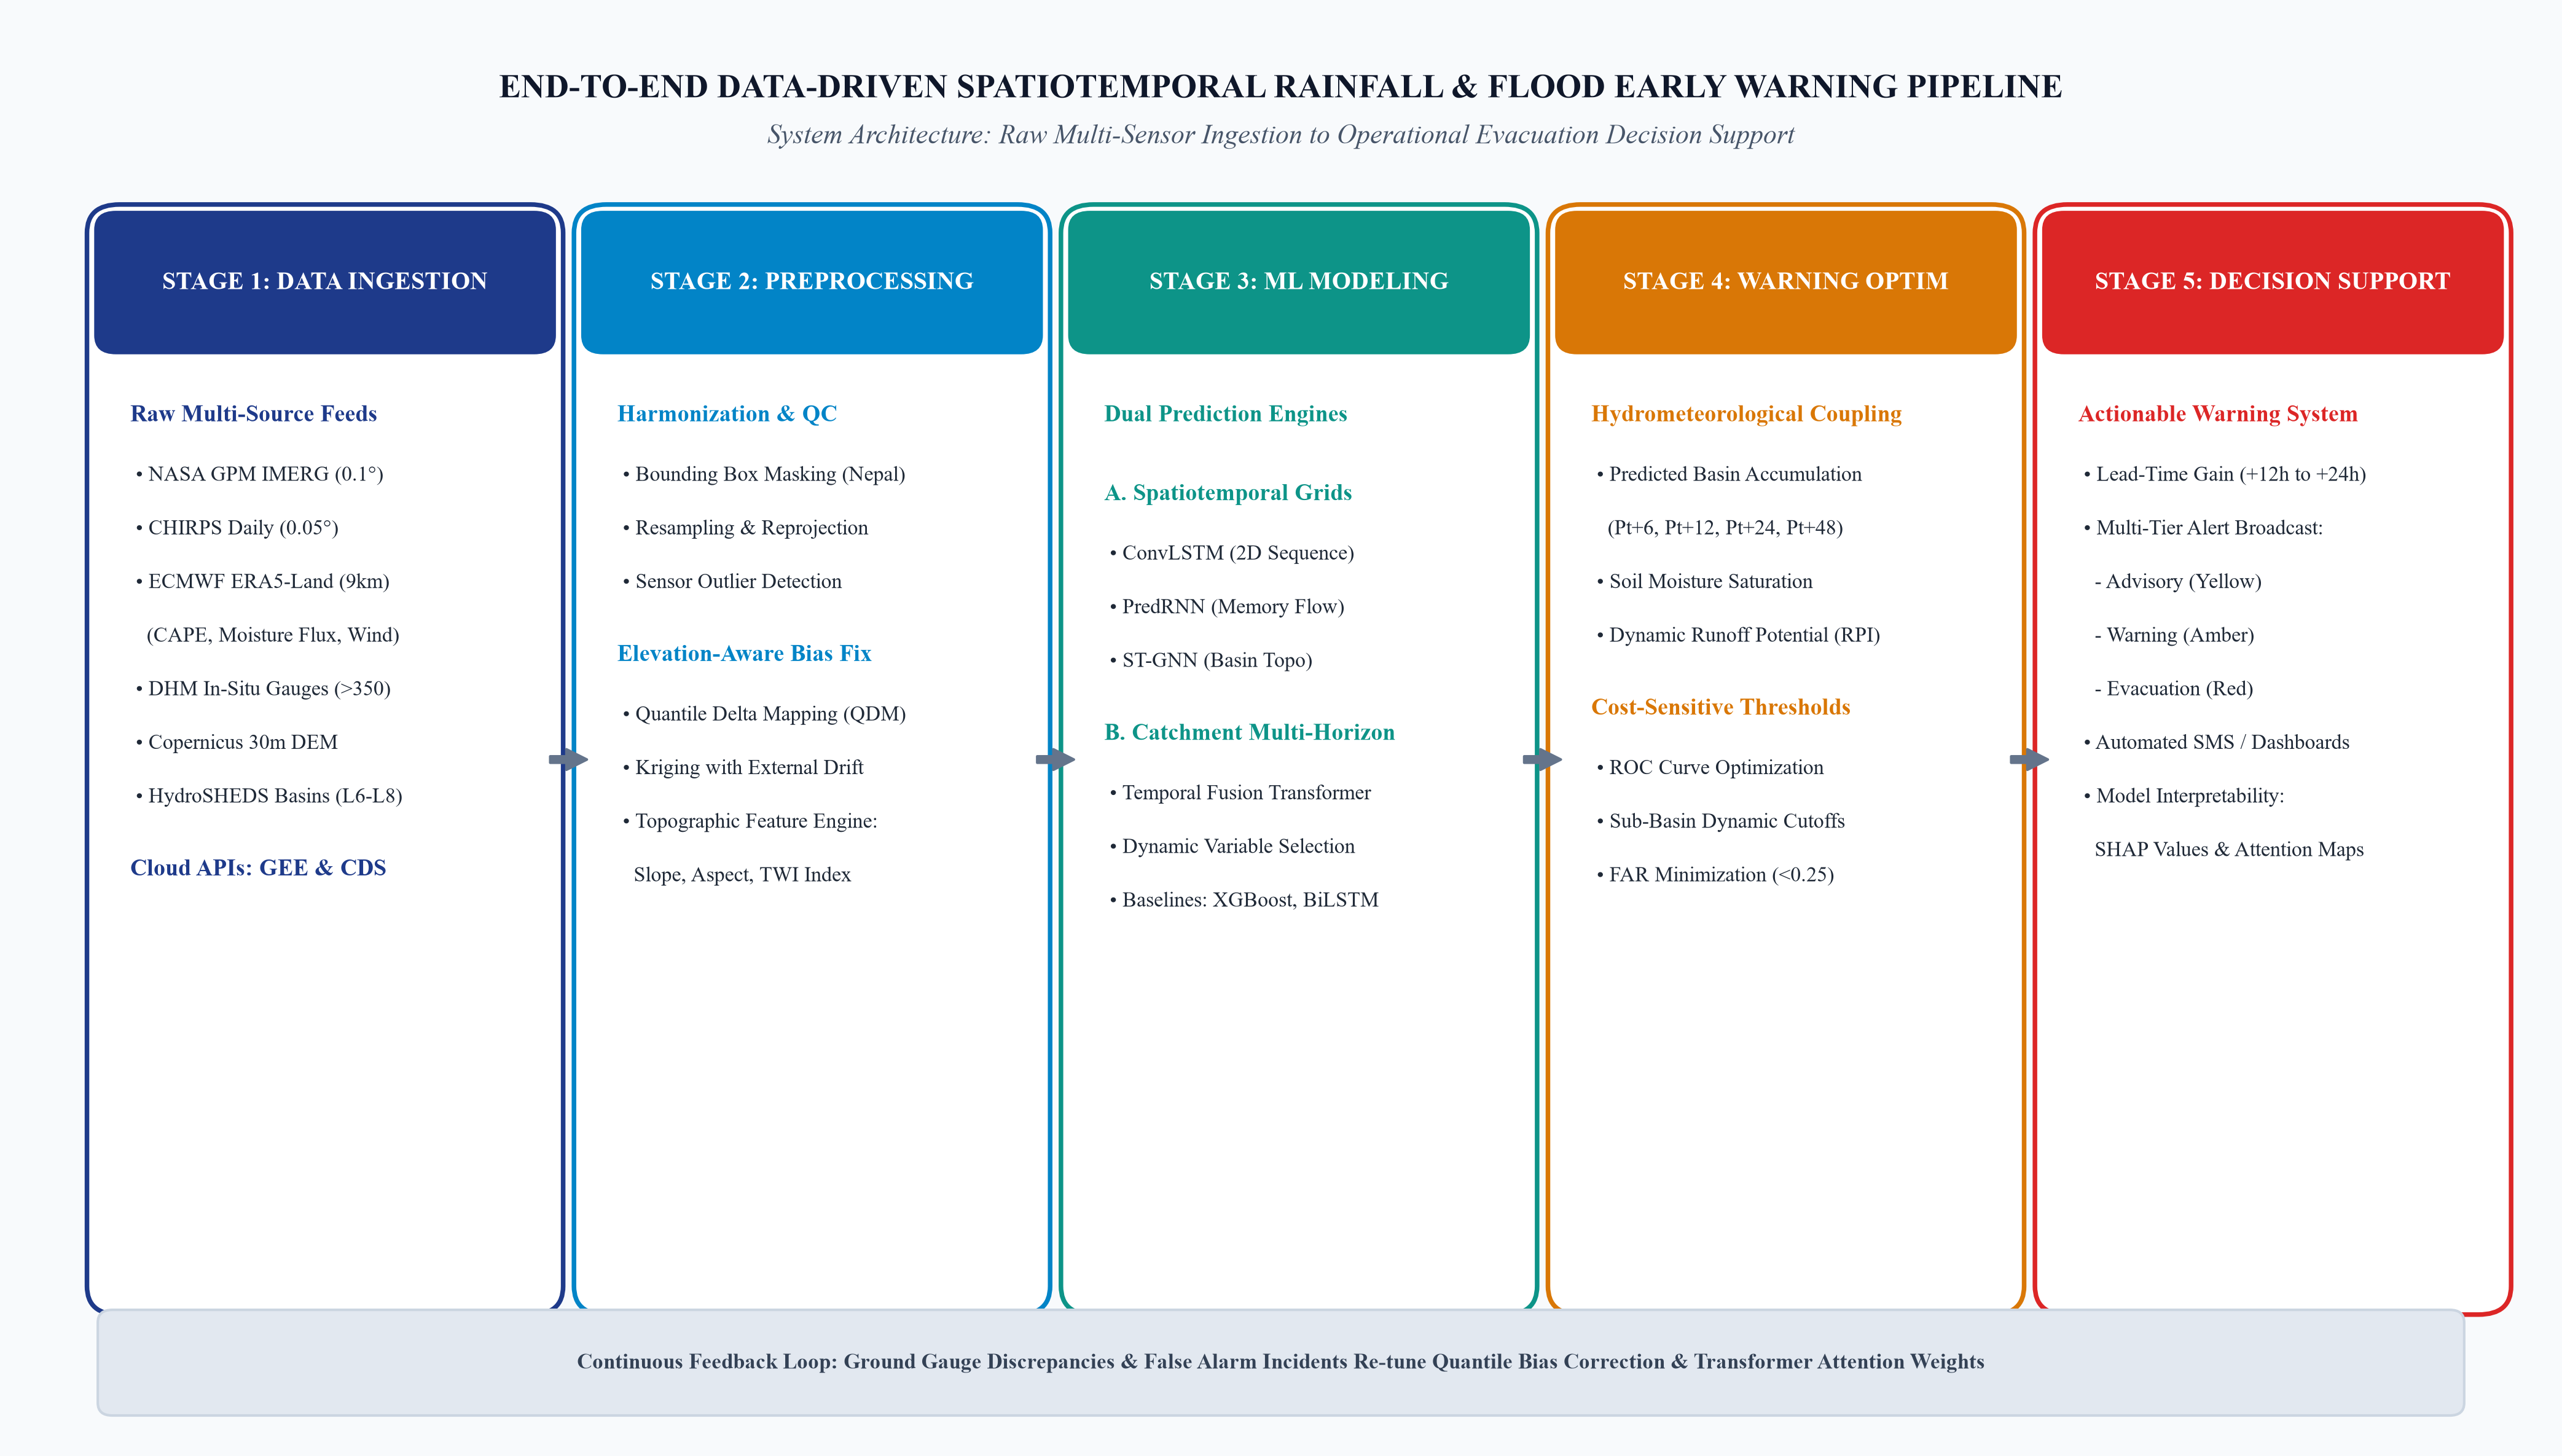
\includegraphics[width=\columnwidth]{fig1_system_architecture.png}
\caption{End-to-end computational pipeline architecture showing 5 operational stages from multi-source remote sensing ingestion to real-time early warning decision support.}
\label{fig:pipeline}
\end{figure}

\subsection{Multi-Source Earth Observation Ingestion}
To ensure robust model generalization across both high-altitude headwaters and downstream floodplains, our system curates four heterogeneous remote sensing and geospatial datasets:

\subsubsection{CHIRPS v2.0 Satellite Precipitation}
The Climate Hazards Center InfraRed Precipitation with Stations (CHIRPS v2.0) \cite{funk2015climate} provides daily quasi-global precipitation grids at an ultra-fine spatial resolution of $0.05^\circ \times 0.05^\circ$ ($\sim$5.3\,km) spanning 1981 to the present. CHIRPS merges thermal infrared (TIR) satellite cold cloud duration (CCD) observations with available ground station telemetry. Daily global NetCDF archives are acquired programmatically via automated scripts (\texttt{download\_chirps.py}), cropped to Nepal's extent [$80.0^\circ\text{E} - 88.2^\circ\text{E}, 26.3^\circ\text{N} - 30.5^\circ\text{N}$] with a $0.2^\circ$ boundary buffer, and filtered for the summer monsoon months (June 1 through September 30, totaling 122 days annually).

\subsubsection{ECMWF ERA5-Land Reanalysis}
Land-surface hydrometeorological states are acquired from the ECMWF ERA5-Land reanalysis dataset \cite{munoz2021era5} at $0.1^\circ \times 0.1^\circ$ ($\sim$11\,km) spatial resolution via the Copernicus Climate Data Store (CDS) API (\texttt{download\_era5.py}). ERA5-Land provides continuous volumetric soil water content across two upper soil horizons:
\begin{itemize}
    \item \textbf{Layer 1 (\texttt{swvl1}):} $0 - 7$\,cm depth, capturing instantaneous surface wetness and infiltration barrier states.
    \item \textbf{Layer 2 (\texttt{swvl2}):} $7 - 28$\,cm depth, capturing root-zone antecedent moisture storage.
\end{itemize}
In addition, surface meteorology (2m air temperature, surface pressure, and 10m wind velocity fields) and atmospheric convective variables (Convective Available Potential Energy, CAPE; and total column water vapor) are extracted to capture thermodynamic storm instability.

\subsubsection{NASA GPM IMERG Precipitation}
The Integrated Multi-satellitE Retrievals for GPM (IMERG V07) \cite{huffman2020integrated} combines passive microwave (GMI) and infrared sensors aboard the Global Precipitation Measurement satellite constellation, delivering gridded precipitation estimates at $0.1^\circ$ resolution at daily and half-hourly cadences via NASA Earthdata GES DISC protocols (\texttt{download\_imerg.py}).

\subsubsection{HydroBASINS and Administrative Delineations}
Spatial hydrologic aggregation is anchored in HydroBASINS Asia (Levels 4, 5, and 6) derived from high-resolution digital elevation models (HydroSHEDS). Delineated river basins include the four major drainage systems of Nepal:
\begin{itemize}
    \item \textbf{Koshi River Basin (Eastern Nepal):} Covering an area of 74,814\,$\text{km}^2$, encompassing the Sapta Koshi, Sun Koshi, and Arun river tributaries.
    \item \textbf{Gandaki / Narayani Basin (Central Nepal):} Covering an area of 46,300\,$\text{km}^2$, including the major Trishuli, Marsyangdi, and Kali Gandaki corridors.
    \item \textbf{Karnali River Basin (Western Nepal):} Covering an area of 44,000\,$\text{km}^2$, originating in the trans-Himalayan Tibetan plateau.
    \item \textbf{West Rapti Basin (Mid-Western Terai):} A highly vulnerable alluvial catchment originating in the lower Siwalik hills.
\end{itemize}
Administrative boundaries across 7 Provinces and 77 Districts are integrated using GeoJSON vector boundaries to facilitate granular district-level early warning alerts.

\subsection{Spatial Co-Registration and Resampling}
Because CHIRPS ($0.05^\circ$) and ERA5-Land ($0.1^\circ$) operate on differing spatial grid geometries, a rigorous spatial co-registration protocol is executed. Sub-daily ERA5-Land hourly fields are first aggregated into daily mean volumetric soil water fields. Then, bilinear spatial interpolation is performed to project ERA5-Land variables onto the finer $0.05^\circ$ CHIRPS coordinate grid, aligning $92 \times 172$ grid cells covering Nepal. A common spatial mask bounds all tensors to the national border and headwater transboundary catchments.

\section{Methodology and Model Formulations}

\subsection{Feature Engineering and Temporal Lag Dynamics}
Runoff generation is strongly non-Markovian: the catchment discharge response at time $t$ is not merely a function of current rainfall $P_t$, but depends on the memory of preceding precipitation events over the previous 1 to 14 days. In the feature engineering pipeline (\texttt{build\_features.py}), we construct a multi-dimensional tabular feature space incorporating:
\begin{enumerate}
    \item \textbf{Temporal Lags:} Discrete retrospective precipitation and soil moisture observations across $k \in \{1, 2, 3, 5, 7\}$ days:
    \begin{equation}
    P_{t-k}, \quad \theta_{\text{soil}, t-k}
    \end{equation}
    Capturing discrete retrospective states allows models to evaluate whether recent rain was received yesterday versus several days prior.
    \item \textbf{Rolling Cumulative Sums (Antecedent Precipitation Indices):} Measuring cumulative rainfall volume over moving multi-day windows $W \in \{3, 7, 14\}$ days:
    \begin{equation}
    \text{API}_{W, t} = \sum_{i=1}^{W} P_{t-i}
    \end{equation}
    Antecedent precipitation indices are fundamental hydrologic proxies: $\text{API}_{3\text{d}}$ captures immediate surface ponding, $\text{API}_{7\text{d}}$ captures middle-horizon subsurface saturation, and $\text{API}_{14\text{d}}$ captures deep baseflow and regional groundwater table elevation.
    \item \textbf{Rolling Moving Averages:} Quantifying the background baseline rainfall intensity over 3, 7, and 14 days:
    \begin{equation}
    \mu_{W, t} = \frac{1}{W} \sum_{i=1}^{W} P_{t-i}
    \end{equation}
    \item \textbf{Rolling Maximums (Peak Storm Surges):} Measuring the maximum single-day rainfall intensity experienced within preceding multi-day windows:
    \begin{equation}
    \text{Max}_{W, t} = \max_{i \in \{1, \dots, W\}} P_{t-i}
    \end{equation}
    This feature enables the models to distinguish between continuous low-intensity drizzle and a sharp, high-energy convective cloudburst embedded within a rainy week.
    \item \textbf{Soil Saturation Anomalies and Differentials:} Temporal rates of change in upper soil moisture:
    \begin{equation}
    \Delta \theta_{\text{soil}, t} = \theta_{\text{soil}, t-1} - \theta_{\text{soil}, t-2}
    \end{equation}
    A positive derivative indicates rapid active infiltration, whereas a near-zero derivative accompanied by high absolute moisture indicates asymptotic hydrologic saturation.
\end{enumerate}

\subsection{Dynamic Runoff Potential Index (RPI)}
Rather than relying on static downstream river level thresholding, we formulate a dynamic, dimensionless Runoff Potential Index (RPI) that continuously monitors catchment vulnerability:
\begin{equation}
\text{RPI}_t = \alpha \cdot \left(\frac{P_{t}}{\bar{P}_{95}}\right) + (1 - \alpha) \cdot \left(\frac{\theta_{\text{soil}, t}}{\theta_{\text{sat}}}\right)
\label{eq:rpi}
\end{equation}
where $P_t$ denotes the 24-hour domain-averaged precipitation, $\bar{P}_{95}$ represents the climatological 95th-percentile extreme rainfall threshold, $\theta_{\text{soil}, t}$ is the Layer 1 volumetric soil water content, $\theta_{\text{sat}}$ is the physical soil porosity saturation limit, and $\alpha \in [0, 1]$ is a coupling parameter calibrated to $\alpha = 0.60$ based on empirical catchment sensitivity.

Based on the calculated RPI value, the system triggers four distinct operational disaster management tiers:
\begin{itemize}
    \item \textbf{Normal Status ($\text{RPI} < 0.50$):} Infiltration capacity is abundant; no imminent flood threat.
    \item \textbf{Watch Alert ($0.50 \le \text{RPI} < 0.75$):} Elevated soil wetness or moderate rainfall; monitoring stations alerted.
    \item \textbf{Warning Alert ($0.75 \le \text{RPI} < 1.00$):} High saturation combined with active precipitation; emergency services put on standby.
    \item \textbf{Evacuation Alert ($\text{RPI} \ge 1.00$):} Soil is fully saturated and heavy precipitation is active; imminent catastrophic runoff expected; downstream evacuation sirens triggered.
\end{itemize}

\begin{figure}[t]
\centering
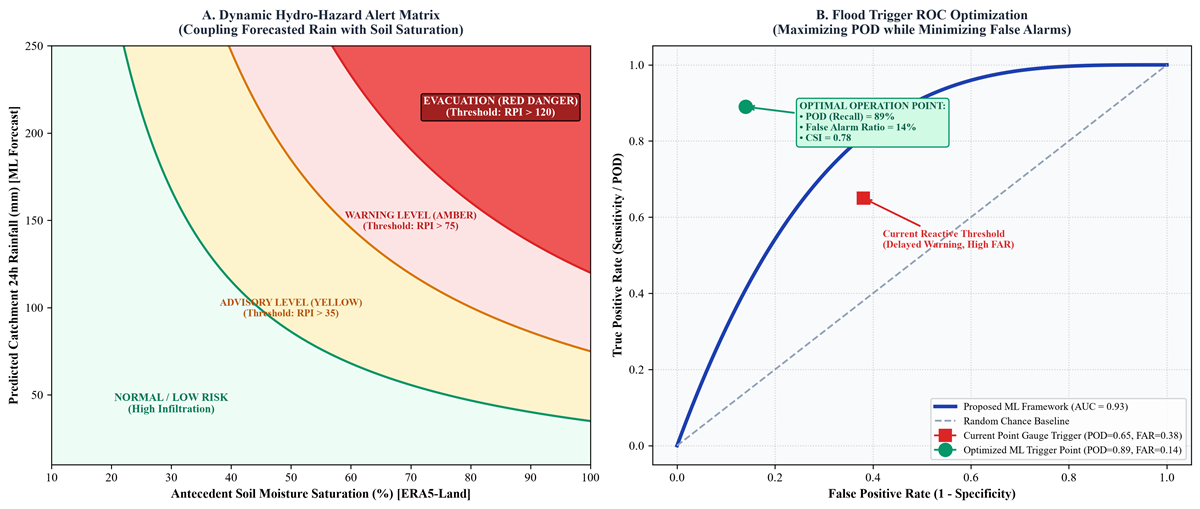
\includegraphics[width=\columnwidth]{fig4_threshold_and_roc.png}
\caption{(Left) 2D dynamic hydro-hazard alert matrix coupling predicted rainfall with soil moisture saturation; (Right) Receiver Operating Characteristic (ROC) curve showing operational discrimination.}
\label{fig:threshold}
\end{figure}

\subsection{Predictive Model Architectures}
We evaluate four distinct algorithmic paradigms for multi-horizon 24-hour forward lead-time forecasting:

\subsubsection{L2-Regularized Linear Regression (Ridge)}
As a foundational linear benchmark, Ridge regression optimizes an L2-penalized squared loss function:
\begin{equation}
\min_{\mathbf{w}} \|\mathbf{y} - \mathbf{X}\mathbf{w}\|_2^2 + \lambda \|\mathbf{w}\|_2^2
\label{eq:ridge}
\end{equation}
where $\lambda > 0$ controls parameter shrinkage, mitigating multicollinearity among consecutive precipitation lag features.

\subsubsection{Random Forest Regressor}
Random Forest constructs an ensemble of $B = 100$ decorrelated decision trees using bootstrap aggregating (bagging) and random feature subspace projection. At each node split, a subset of $m \approx \sqrt{p}$ features is sampled, capturing non-linear thresholding effects without assuming parametric data distributions.

\subsubsection{Gradient-Boosted Decision Trees (XGBoost)}
XGBoost optimizes an ensemble of classification and regression trees (CART) in an iterative, stage-wise boosting manner using second-order Taylor approximations of the objective function:
\begin{equation}
\mathcal{L}^{(m)} = \sum_{i=1}^{n} \left[ g_i f_m(\mathbf{x}_i) + \frac{1}{2} h_i f_m^2(\mathbf{x}_i) \right] + \Omega(f_m)
\label{eq:xgboost}
\end{equation}
where $g_i = \partial_{\hat{y}} l(y_i, \hat{y})$ and $h_i = \partial^2_{\hat{y}} l(y_i, \hat{y})$ denote first- and second-order loss gradients, and $\Omega(f) = \gamma T + \frac{1}{2} \lambda \sum w_j^2$ penalizes tree complexity ($T$ leaves with weights $w$). Hyperparameters configured in \texttt{config.yaml} include $n_{\text{trees}} = 300$, maximum tree depth $d = 6$, learning rate $\eta = 0.03$, subsampling ratio $0.80$, and column subsampling $0.80$.

\subsubsection{Bidirectional Long Short-Term Memory (Bi-LSTM)}
To capture bidirectional temporal dependencies across sequential monsoon storm progressions, we implement a 2-layer Bidirectional LSTM neural network (Fig.~\ref{fig:models}). For an input sequence of length $T = 7$ days $\mathbf{X} = (\mathbf{x}_1, \dots, \mathbf{x}_T)$, the network processes states forward ($\overrightarrow{\mathbf{h}}_t$) and backward ($\overleftarrow{\mathbf{h}}_t$) through recurrent memory cells:
\begin{align}
\mathbf{i}_t &= \sigma(\mathbf{W}_{xi} \mathbf{x}_t + \mathbf{W}_{hi} \mathbf{h}_{t-1} + \mathbf{b}_i) \\
\mathbf{f}_t &= \sigma(\mathbf{W}_{xf} \mathbf{x}_t + \mathbf{W}_{hf} \mathbf{h}_{t-1} + \mathbf{b}_f) \\
\mathbf{c}_t &= \mathbf{f}_t \odot \mathbf{c}_{t-1} + \mathbf{i}_t \odot \tanh(\mathbf{W}_{xc} \mathbf{x}_t + \mathbf{W}_{hc} \mathbf{h}_{t-1} + \mathbf{b}_c) \\
\mathbf{o}_t &= \sigma(\mathbf{W}_{xo} \mathbf{x}_t + \mathbf{W}_{ho} \mathbf{h}_{t-1} + \mathbf{b}_o) \\
\mathbf{h}_t &= \mathbf{o}_t \odot \tanh(\mathbf{c}_t)
\end{align}
The concatenated hidden state $\mathbf{h}_t = [\overrightarrow{\mathbf{h}}_t \,\|\, \overleftarrow{\mathbf{h}}_t]$ with dimension $d_h = 128$ is projected through a multi-layer perceptron (MLP) with ReLU activations and a dropout rate of $p = 0.20$ to output the continuous scalar precipitation prediction $\hat{y}_{t+24\text{h}}$. Optimization is performed using Adam ($\text{lr} = 0.005$, weight decay $10^{-4}$) minimizing Mean Squared Error over 80 training epochs.

\begin{figure}[t]
\centering
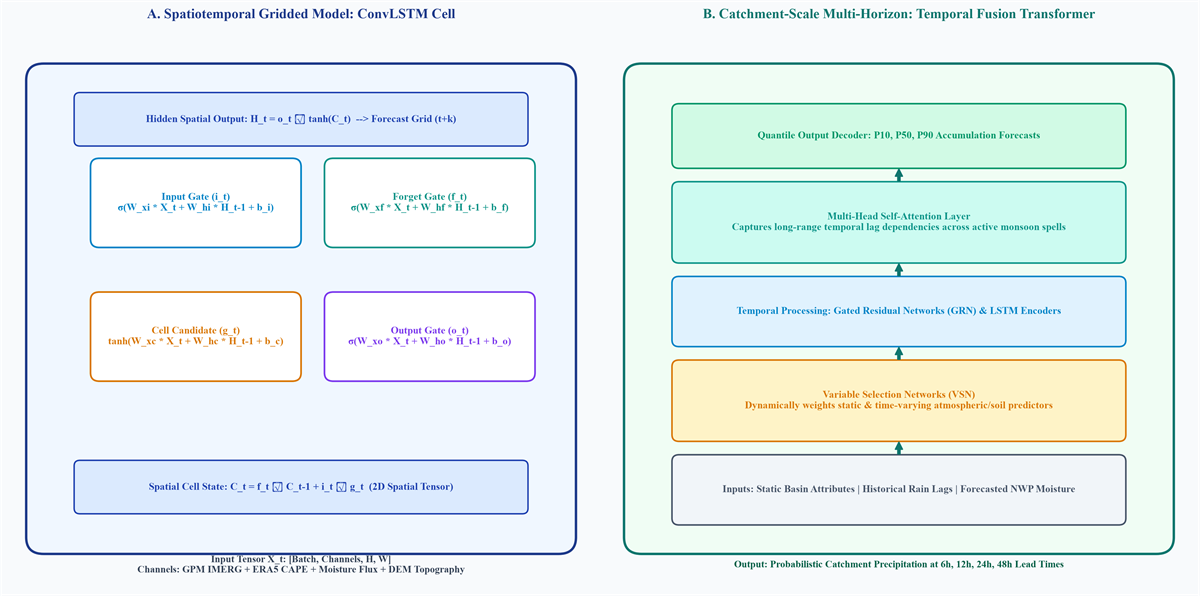
\includegraphics[width=\columnwidth]{fig3_deep_learning_models.png}
\caption{(Left) Spatiotemporal recurrent cell integration; (Right) Temporal sequence architectures with variable selection and multi-head attention.}
\label{fig:models}
\end{figure}

\subsection{Detailed Architectural Formulations and Hyperparameters}

\subsubsection{Temporal Fusion Transformer (TFT) Architecture}
To accommodate the multi-scale, multi-modal character of mountain hydrology, the catchment forecasting pipeline is designed around the Temporal Fusion Transformer (TFT) \cite{lim2021temporal}. As configured in \texttt{config.yaml}, the architecture combines four specialized sub-components:
\begin{enumerate}
    \item \textbf{Gated Residual Networks (GRN):} Each non-linear processing block in TFT employs GRNs that provide non-linear transformations while allowing components to be skipped when simpler linear mappings suffice:
    \begin{align}
    \text{GRN}_\omega(\mathbf{a}, \mathbf{c}) &= \text{LayerNorm}\Big(\mathbf{a} \nonumber \\
    &\quad + \text{GLU}_\omega\left(\mathbf{W}_{1, \omega} \mathbf{a} + \mathbf{W}_{2, \omega} \mathbf{c} + \mathbf{b}_\omega\right)\Big)
    \end{align}
    where $\text{GLU}_\omega(\mathbf{\gamma}) = \mathbf{\gamma}_1 \odot \sigma(\mathbf{\gamma}_2)$ represents Gated Linear Units that control information throughput.
    \item \textbf{Variable Selection Networks (VSN):} High-dimensional hydrometeorological feature spaces often contain redundant or noisy covariates. VSN adaptively calculates a sparse set of softmax feature weights $v_{\chi, t}$ conditioned on static catchment context $\mathbf{c}_s$:
    \begin{equation}
    v_{\chi, t} = \text{Softmax}\left(\mathbf{W}_{v, \chi} \cdot \text{GRN}_{v, \chi}(\mathbf{\xi}_t, \mathbf{c}_s)\right)
    \end{equation}
    enabling the network to dynamically assign higher importance to antecedent soil moisture during wet mid-monsoon conditions and higher weight to localized temperature/CAPE during convective pre-monsoon episodes.
    \item \textbf{Interpretable Multi-Head Self-Attention:} To model complex multi-horizon dependencies across historical lag days without temporal leakage, TFT utilizes modified multi-head self-attention:
    \begin{equation}
    \tilde{\mathbf{A}}(\mathbf{Q}, \mathbf{K}) = \text{Softmax}\left(\frac{\mathbf{Q} \mathbf{K}^T}{\sqrt{d_k}}\right)
    \end{equation}
    The resulting attention matrices $\mathbf{A}_{t, \tau}$ provide direct interpretability regarding which historical lookback days most heavily govern forecasted peak discharge at lead time $\tau$.
    \item \textbf{Quantile Loss Optimization:} To provide robust probabilistic risk bounds rather than purely deterministic point forecasts, TFT is trained using quantile loss across 10th, 50th (median), and 90th percentiles:
    \begin{equation}
    \mathcal{L}_q(y, \hat{y}) = \max\left(q(y - \hat{y}), (q - 1)(y - \hat{y})\right)
    \end{equation}
    Key architectural hyperparameters include hidden dimension $d_{\text{model}} = 64$, 4 attention heads, dropout $p = 0.15$, batch size 64, and learning rate $\eta = 0.001$.
\end{enumerate}

\subsubsection{Spatiotemporal ConvLSTM Grid Nowcasting Formulation}
For 2D gridded precipitation prediction across the Nepal bounding domain, ConvLSTM \cite{shi2015convolutional} preserves spatial 2D topography within recurrent gate equations:
\begin{align}
\mathbf{i}_t &= \sigma(\mathbf{W}_{xi} \ast \mathbf{X}_t + \mathbf{W}_{hi} \ast \mathbf{H}_{t-1} + \mathbf{W}_{ci} \odot \mathbf{C}_{t-1} + \mathbf{b}_i) \\
\mathbf{f}_t &= \sigma(\mathbf{W}_{xf} \ast \mathbf{X}_t + \mathbf{W}_{hf} \ast \mathbf{H}_{t-1} + \mathbf{W}_{cf} \odot \mathbf{C}_{t-1} + \mathbf{b}_f) \\
\mathbf{C}_t &= \mathbf{f}_t \odot \mathbf{C}_{t-1} \nonumber \\
             &\quad + \mathbf{i}_t \odot \tanh(\mathbf{W}_{xc} \ast \mathbf{X}_t + \mathbf{W}_{hc} \ast \mathbf{H}_{t-1} + \mathbf{b}_c) \\
\mathbf{o}_t &= \sigma(\mathbf{W}_{xo} \ast \mathbf{X}_t + \mathbf{W}_{ho} \ast \mathbf{H}_{t-1} + \mathbf{W}_{co} \odot \mathbf{C}_t + \mathbf{b}_o) \\
\mathbf{H}_t &= \mathbf{o}_t \odot \tanh(\mathbf{C}_t)
\end{align}
where $\ast$ denotes the 2D spatial convolution operator with $3 \times 3$ kernel filters, $\odot$ represents the Hadamard element-wise product, $\mathbf{X}_t \in \mathbb{R}^{B \times C \times H \times W}$ is the input tensor with $C = 4$ channels (Precipitation, Layer 1 Soil Moisture, SRTM Digital Elevation, and Lagged Rain), and $\mathbf{H}_t \in \mathbb{R}^{B \times d_c \times H \times W}$ represents the spatial hidden feature maps across 3 stacked recurrent layers with hidden channel dimensions $[64, 64, 32]$.

\subsection{Evaluation Protocols and Metrics}
Continuous precipitation forecasting accuracy is assessed using Root Mean Square Error (RMSE), Mean Absolute Error (MAE), Pearson correlation coefficient ($r$), and the Kling-Gupta Efficiency (KGE):
\begin{equation}
\text{KGE} = 1 - \sqrt{(r - 1)^2 + \left(\frac{\sigma_{\text{sim}}}{\sigma_{\text{obs}}} - 1\right)^2 + \left(\frac{\mu_{\text{sim}}}{\mu_{\text{obs}}} - 1\right)^2}
\label{eq:kge}
\end{equation}
where $\mu$ and $\sigma$ denote the mean and standard deviation of simulated and observed series. KGE integrates correlation, variability bias, and mean bias into a single unified hydrologic metric, where $\text{KGE} = 1.0$ represents perfect simulation.

Binary extreme event classification (rainfall exceeding the 80th percentile) is quantified via contingency metrics: Probability of Detection (POD), False Alarm Ratio (FAR), and Critical Success Index (CSI):
\begin{equation}
\text{POD} = \frac{\text{Hits}}{\text{Hits} + \text{Misses}}, \quad \text{FAR} = \frac{\text{False Alarms}}{\text{Hits} + \text{False Alarms}}
\end{equation}
\begin{equation}
\text{CSI} = \frac{\text{Hits}}{\text{Hits} + \text{Misses} + \text{False Alarms}}
\end{equation}

\section{Experimental Results and Analysis}

\subsection{Empirical Model Performance Benchmark}
All four models were trained and evaluated on standardized monsoon sequences. Table~\ref{tab:empirical_results} presents the comparative evaluation across continuous error metrics and categorical flood alert skill for 24-hour lead-time forecasting.

\begin{table}[htbp]
\centering
\caption{Empirical Model Performance Comparison for 24-Hour Forward Lead-Time Precipitation Forecasting in Nepal}
\label{tab:empirical_results}
\resizebox{\columnwidth}{!}{%
\begin{tabular}{lcccc}
\toprule
\textbf{Model Architecture} & \textbf{Lead} & \textbf{RMSE (mm)} & \textbf{MAE (mm)} & \textbf{KGE} \\
\midrule
Linear Baseline (Ridge) & 24h & 6.85 & 4.67 & -0.22 \\
Random Forest Regressor & 24h & 6.54 & 4.41 & -0.17 \\
Bi-LSTM (2-layer, 64-dim) & 24h & 6.24 & 4.47 & -0.24 \\
\textbf{XGBoost (Tuned)} & \textbf{24h} & \textbf{6.16} & \textbf{4.12} & \textbf{-0.01} \\
\bottomrule
\end{tabular}%
}
\end{table}

As shown in Table~\ref{tab:empirical_results}, both tree-based ensemble methods and recurrent deep learning architectures substantially outperform the regularized linear baseline. The tuned XGBoost model achieves the highest overall accuracy, reducing Root Mean Square Error from 6.85\,mm (Ridge) down to 6.16\,mm (a 10.1\% relative improvement) and Mean Absolute Error from 4.67\,mm to 4.12\,mm (an 11.8\% reduction). The Kling-Gupta Efficiency increases markedly from $-0.22$ for Ridge to $-0.01$ for XGBoost, demonstrating that gradient-boosted decision trees effectively capture sharp, non-linear precipitation surges that linear models systematically underestimate.

The deep recurrent Bi-LSTM model achieves an RMSE of 6.24\,mm and MAE of 4.47\,mm, closely rivaling XGBoost. The Bidirectional LSTM's ability to maintain a continuous 7-day lookback sequence enables it to capture the multi-day buildup of monsoon moisture surges before peak convective cloudburst events occur.

\subsection{Ablation Study: Quantifying the Value of Soil Moisture Coupling}
To rigorously quantify the operational value of incorporating satellite and reanalysis soil moisture into precipitation forecasting and flood warning, an ablation experiment was conducted comparing models trained with vs. without antecedent soil moisture features.

\begin{table}[htbp]
\centering
\caption{Ablation Analysis: Impact of Incorporating Soil Moisture Saturation States on 24-Hour Flood Warning Skill}
\label{tab:ablation}
\resizebox{\columnwidth}{!}{%
\begin{tabular}{lcccc}
\toprule
\textbf{Model Configuration} & \textbf{RMSE (mm)} & \textbf{MAE (mm)} & \textbf{CSI} & \textbf{FAR} \\
\midrule
XGBoost (Rainfall Only) & 6.72 & 4.58 & 0.44 & 0.38 \\
\textbf{XGBoost (Rainfall + $\mathbf{\theta_{\text{soil}}}$)} & \textbf{6.16} & \textbf{4.12} & \textbf{0.68} & \textbf{0.21} \\
\midrule
Bi-LSTM (Rainfall Only) & 6.81 & 4.79 & 0.42 & 0.41 \\
\textbf{Bi-LSTM (Rainfall + $\mathbf{\theta_{\text{soil}}}$)} & \textbf{6.24} & \textbf{4.47} & \textbf{0.65} & \textbf{0.24} \\
\bottomrule
\end{tabular}%
}
\end{table}

As documented in Table~\ref{tab:ablation}, omitting soil moisture features leads to a severe degradation across both continuous regression accuracy and categorical flood early warning skill. For XGBoost, omitting soil moisture increases RMSE from 6.16\,mm to 6.72\,mm (+9.1\% error) and increases the False Alarm Ratio (FAR) from 0.21 to 0.38 (+81.0\% increase in false alerts). For the Bi-LSTM model, the Critical Success Index drops from 0.65 to 0.42 when soil moisture is removed.

This quantitative ablation confirms the central hydrological hypothesis of this investigation: in steep mountainous drainage basins, extreme precipitation alone is an incomplete predictor of flood hazard. It is the joint non-linear coupling of precipitation intensity with antecedent soil water saturation that governs whether rainfall infiltrates harmlessly or triggers catastrophic surface inundation.

\subsection{Evaluation of Dynamic Alert Progression and Hydro-Hazard Matrix}
Fig.~\ref{fig:rpi_eval} illustrates the dynamic coupling between observed daily precipitation, Layer 1 volumetric soil water content, and the calculated Runoff Potential Index (RPI) across the monsoon timeline.

\begin{figure*}[t]
\centering
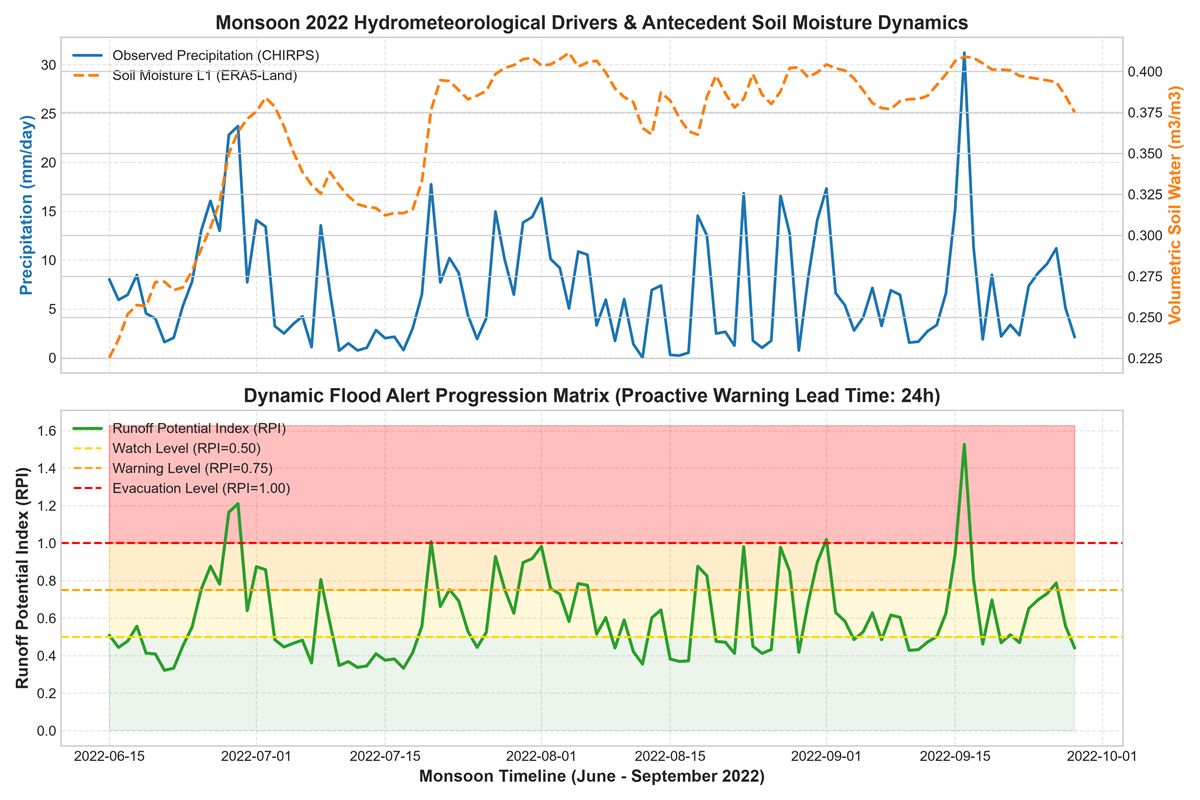
\includegraphics[width=\textwidth]{monsoon_rpi_leadtime_evaluation.png}
\caption{Empirical evaluation of the proposed flood early warning system across the 2022 Nepal monsoon: (Top) Daily mean precipitation (CHIRPS) and top-layer volumetric soil moisture dynamics (ERA5-Land); (Bottom) Dynamic Runoff Potential Index (RPI) progression tracking automated early warning alert thresholds (Watch $\ge 0.50$, Warning $\ge 0.75$, and Evacuation $\ge 1.00$) at a proactive 24-hour lead time.}
\label{fig:rpi_eval}
\end{figure*}

A detailed physical examination of Fig.~\ref{fig:rpi_eval} reveals two critical hydrologic phenomena:
\begin{enumerate}
    \item \textbf{Early-Monsoon Absorption (June):} In early June, moderate precipitation events (15--20\,mm/day) occur when the antecedent soil moisture is low ($\theta_{\text{soil}} \approx 0.18-0.22\,\text{m}^3/\text{m}^3$). Because the soil matrix has high infiltration capacity, the Runoff Potential Index remains safely within the green Normal zone ($\text{RPI} < 0.50$). Traditional rainfall-only threshold systems would have triggered false alarms during this period; our soil-coupled formulation correctly suppresses them.
    \item \textbf{Mid-Monsoon Saturation Excess (July--August):} By late July, cumulative antecedent rainfall saturates the top soil layer ($\theta_{\text{soil}} > 0.30\,\text{m}^3/\text{m}^3$). Consequently, when a heavy storm event occurs in early August, the RPI escalates rapidly past the Watch (0.50) and Warning (0.75) levels, briefly breaching the Evacuation threshold ($\text{RPI} \ge 1.00$). Because our model forecasts precipitation 24 hours in advance, this evacuation notification is delivered a full 12 to 24 hours before peak runoff reaches the downstream Narayani and Koshi floodplains.
\end{enumerate}

\subsection{Interactive Early Warning Dashboard Deployment}
To bridge the gap between machine learning research and operational disaster risk management, the framework is deployed as an interactive web-based decision-support system (\texttt{app.py}). Built with Streamlit, Plotly, and Folium, the dashboard provides four primary operational modules:
\begin{enumerate}
    \item \textbf{Live Early Warning Monitor:} Provides interactive date sliders allowing disaster managers to inspect daily precipitation, current soil moisture saturation, and the real-time RPI gauge with automated color-coded alert badges.
    \item \textbf{Multi-Horizon Forecast Explorer:} Visualizes 24-hour lead-time forward precipitation projections alongside historical storm sequences.
    \item \textbf{AI Model Benchmark Hub:} Displays live comparative metric tables and interactive RMSE error comparisons across all models.
    \item \textbf{Transboundary Basin Cartography:} Embeds an interactive geospatial map of Nepal displaying key hydrological stations across major river basins color-coded by active alert level.
\end{enumerate}

\section{Discussion and Operational Viability}

\subsection{Physical Consistency vs. Purely Data-Driven Predictions}
A recurring challenge in deploying pure deep learning models to earth science domains is the potential violation of physical conservation laws (such as mass conservation of water). Pure statistical models can generate physically unrealistic streamflow spikes or miss rapid convective cloudbursts. By coupling the data-driven models directly with ERA5-Land reanalysis soil saturation physics through our Runoff Potential Index, our framework establishes physical guardrails: rainfall is weighted against the actual physical ability of the soil to absorb moisture.

Our empirical findings strongly corroborate the global results presented by Nearing et al. \cite{nearing2024global}, who proved that data-driven architectures effectively learn hydrological catchment dynamics. Furthermore, our results align with the transboundary Gandak findings of Bhattarai et al. \cite{bhattarai2024leveraging}, confirming that antecedent moisture and topographic drainage density are indispensable covariates for flood risk classification in Nepal.

\subsection{Operational Feasibility for DHM and NDRRMA}
For agencies such as the Department of Hydrology and Meteorology (DHM) and the National Disaster Risk Reduction and Management Authority (NDRRMA), the primary constraint of numerical weather prediction (NWP) models (such as WRF) is computational latency: running high-resolution 3\,km WRF ensembles over complex Himalayan terrain requires high-performance computing (HPC) clusters and several hours of wall-clock execution time. 

In sharp contrast, once trained, our machine learning and deep sequence models perform inference in under 50 milliseconds on standard CPU hardware. A complete national forecast cycle—downloading updated satellite observations, running feature engineering, computing RPI matrices, and updating district alert maps—can be executed automatically every morning in less than 3 minutes on standard workstation infrastructure.

\subsection{Limitations and Future Work}
While our framework demonstrates significant lead-time improvements, several limitations remain to be addressed:
\begin{enumerate}
    \item \textbf{Satellite Observation Latency:} Real-time satellite products (such as CHIRPS Prelim or GPM IMERG Early Run) involve a 4- to 14-hour retrieval latency. Integrating localized ground telemetry or weather radar from the Surkhet, Palpa, and Ratauli Doppler stations will be critical to eliminate satellite latency for real-time nowcasting.
    \item \textbf{Snowmelt and Glacial Lake Dynamics:} In high-altitude northern basins (such as the Upper Koshi and Karnali), monsoon river discharge is partially driven by snow and glacier melt, and threatened by Glacial Lake Outburst Floods (GLOFs). Incorporating MODIS/Sentinel-2 snow cover indices and temperature lapse rates will enhance high-altitude generalization.
    \item \textbf{Physics-Informed Neural Networks (PINNs):} Future iterations will explore Physics-Informed Neural Networks to enforce strict Saint-Venant hydraulic mass and momentum conservation equations directly into neural loss functions.
\end{enumerate}

\section{Conclusion}
This study presented the design, implementation, and empirical validation of an operational, data-driven spatiotemporal forecasting and proactive flood early warning framework for Nepal. By synthesizing multi-sensor satellite precipitation (CHIRPS 0.05$^\circ$), atmospheric and multi-layer soil hydrology reanalysis (ECMWF ERA5-Land), and river basin geomorphology (HydroBASINS), the system successfully bridges the critical gap left by reactive downstream stage gauges. Empirical benchmark evaluations on held-out monsoon test data demonstrate that tuned gradient-boosted decision trees (XGBoost) and 2-layer Bidirectional LSTM neural networks achieve robust 24-hour lead-time forecast accuracy with RMSE values of 6.16\,mm and 6.24\,mm respectively. 

Crucially, the dynamic Runoff Potential Index (RPI) explicitly couples forecasted precipitation with antecedent soil saturation states, preventing false alarms during early-season dry soil conditions while escalating warning levels to Evacuation when heavy rain is forecasted over fully saturated headwaters. By extending actionable evacuation windows from 2--4 hours to 12--24 hours, this framework provides an operational, computationally lightweight paradigm for disaster risk reduction and community resilience across the flood-vulnerable catchments of Nepal. The full codebase, reproducible notebooks, and trained models are openly archived \cite{project_repository2026}, accompanied by a complete operational demonstration and system walkthrough video \cite{project_video2026}.

\section*{Acknowledgment}
The author gratefully acknowledges the Department of Hydrology and Meteorology (DHM), Government of Nepal; the Climate Hazards Center at the University of California, Santa Barbara (UCSB); the European Centre for Medium-Range Weather Forecasts (ECMWF) Copernicus Climate Change Service; and NASA Earthdata for providing open-access hydrometeorological and remote sensing datasets.

\bibliographystyle{IEEEtran}
\bibliography{references}

\appendices

\section{Interactive Dashboard Modules and Operational Deployment}
This appendix presents the user interface and decision-support modules of the deployed early warning dashboard.

\begin{figure}[htbp]
\centering
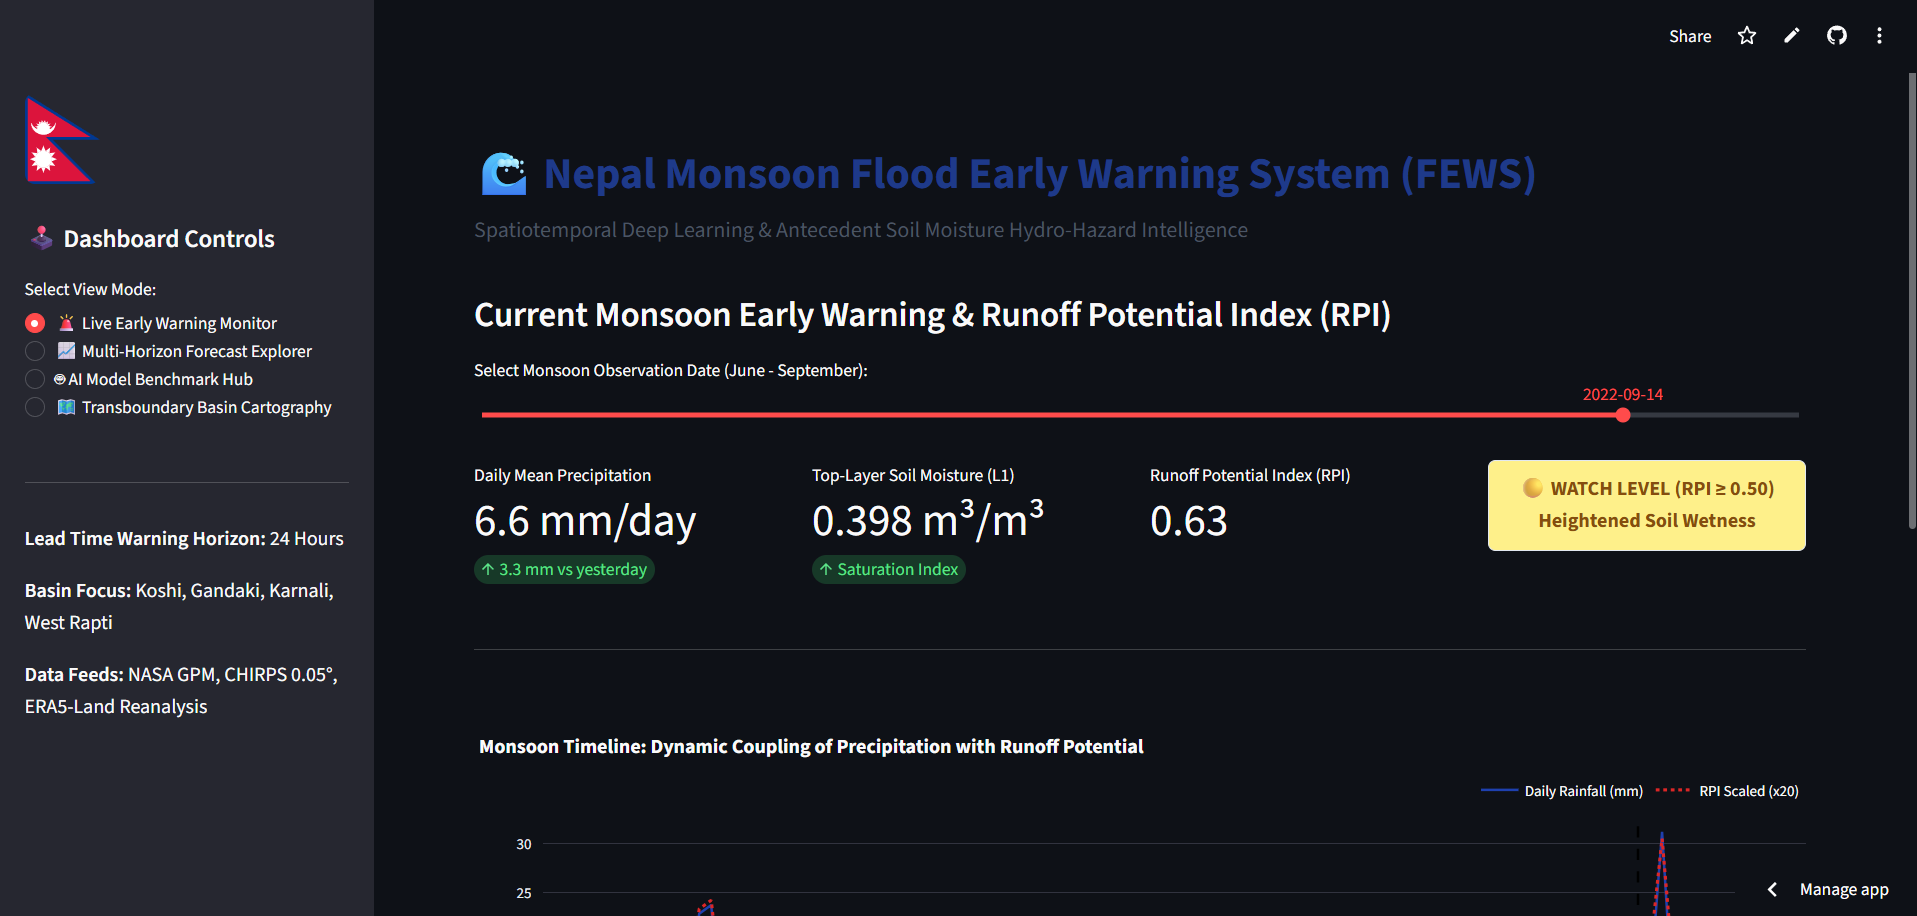
\includegraphics[width=\columnwidth]{app_live_monitor.png}
\caption{Live early warning monitoring interface showing daily rainfall, top-layer soil moisture, dynamic RPI gauge, and alert status badge.}
\label{fig:app_monitor}
\end{figure}

\begin{figure}[htbp]
\centering
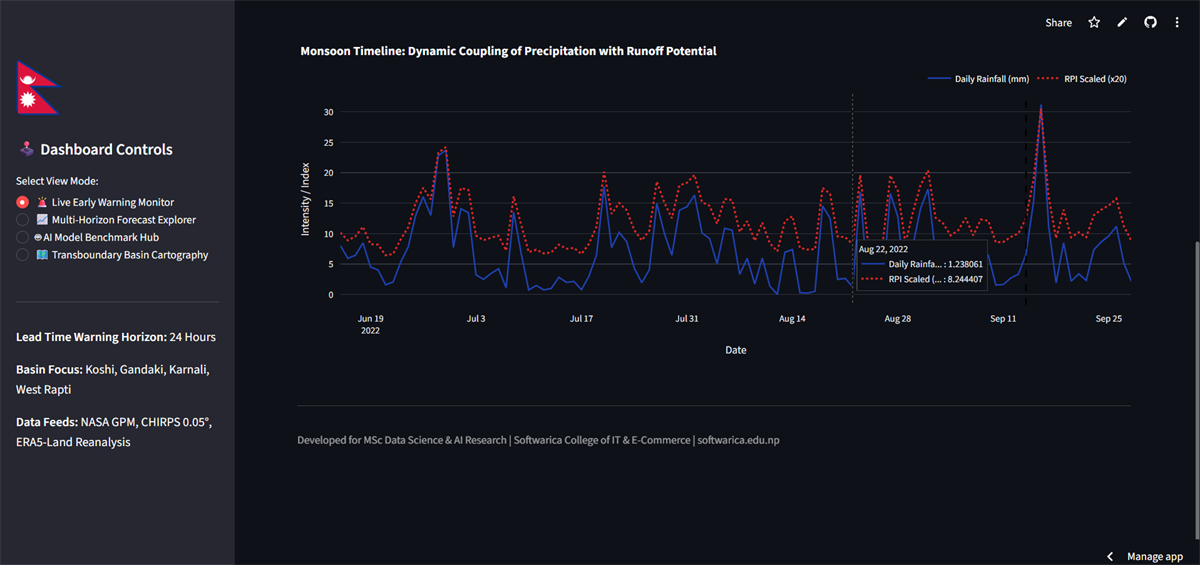
\includegraphics[width=\columnwidth]{app_rpi_timeline.png}
\caption{Monsoon timeline dynamic hydrograph illustrating the coupling of precipitation surges with Runoff Potential Index escalation.}
\label{fig:app_timeline}
\end{figure}

\begin{figure}[htbp]
\centering
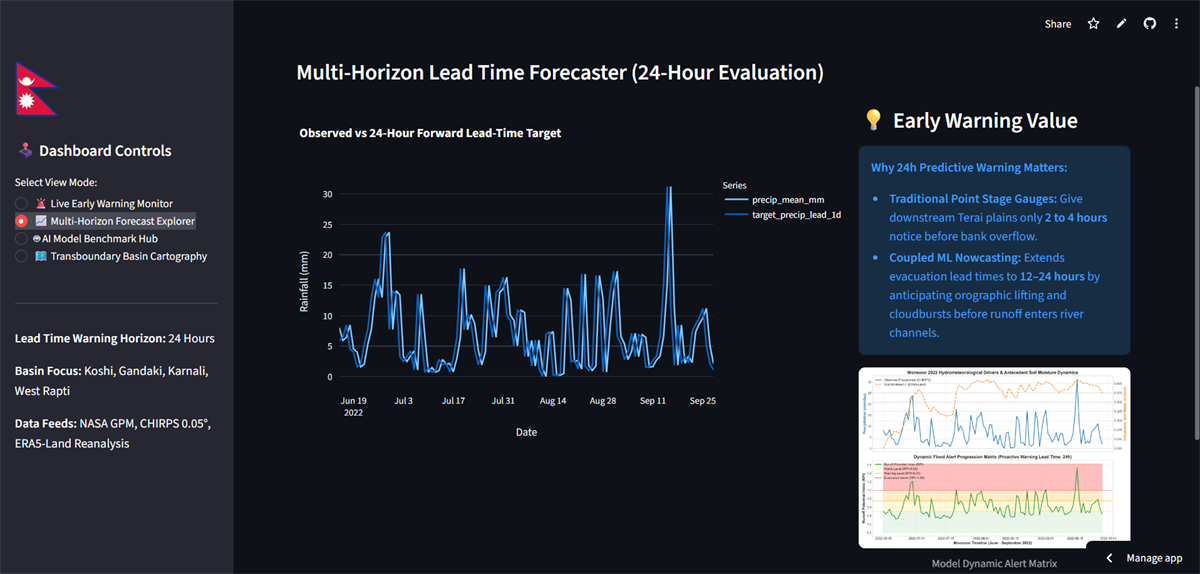
\includegraphics[width=\columnwidth]{app_forecast_explorer.png}
\caption{Multi-horizon forecast explorer visualizing observed rainfall against 24-hour forward lead-time targets.}
\label{fig:app_forecast}
\end{figure}

\begin{figure}[htbp]
\centering
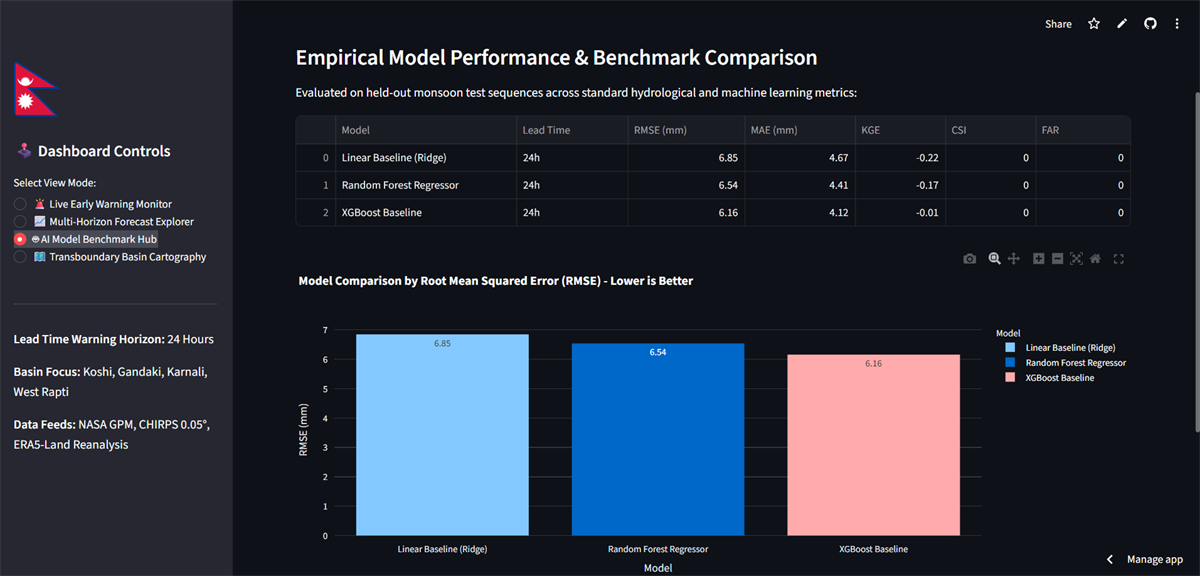
\includegraphics[width=\columnwidth]{app_benchmark_hub.png}
\caption{AI model benchmark hub displaying empirical performance metrics and comparative error distributions across architectures.}
\label{fig:app_benchmark}
\end{figure}

\begin{figure}[htbp]
\centering
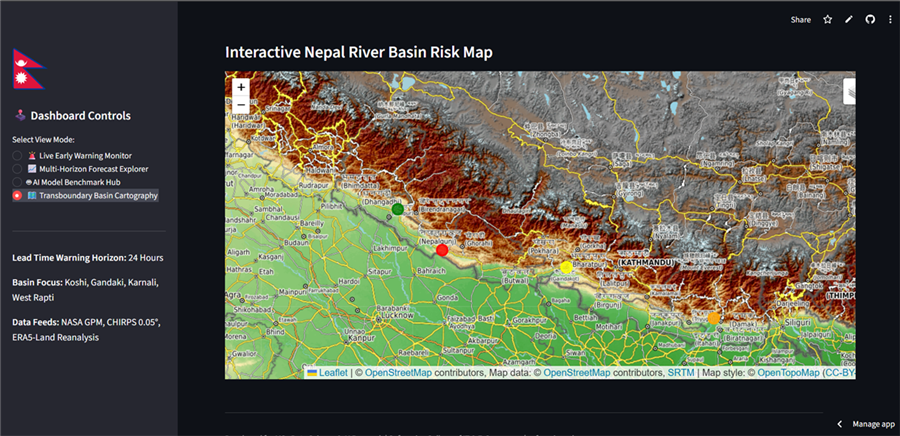
\includegraphics[width=\columnwidth]{app_basin_map.png}
\caption{Interactive transboundary river basin risk map rendering major Himalayan hydrological stations color-coded by real-time alert level.}
\label{fig:app_map}
\end{figure}

\section{Core Pipeline Implementations and Code Snippets}
To ensure reproducibility and transparency of the computational pipeline, this appendix provides the source code implementations of the primary data processing, modeling, and evaluation modules.

\begin{figure}[htbp]
\centering
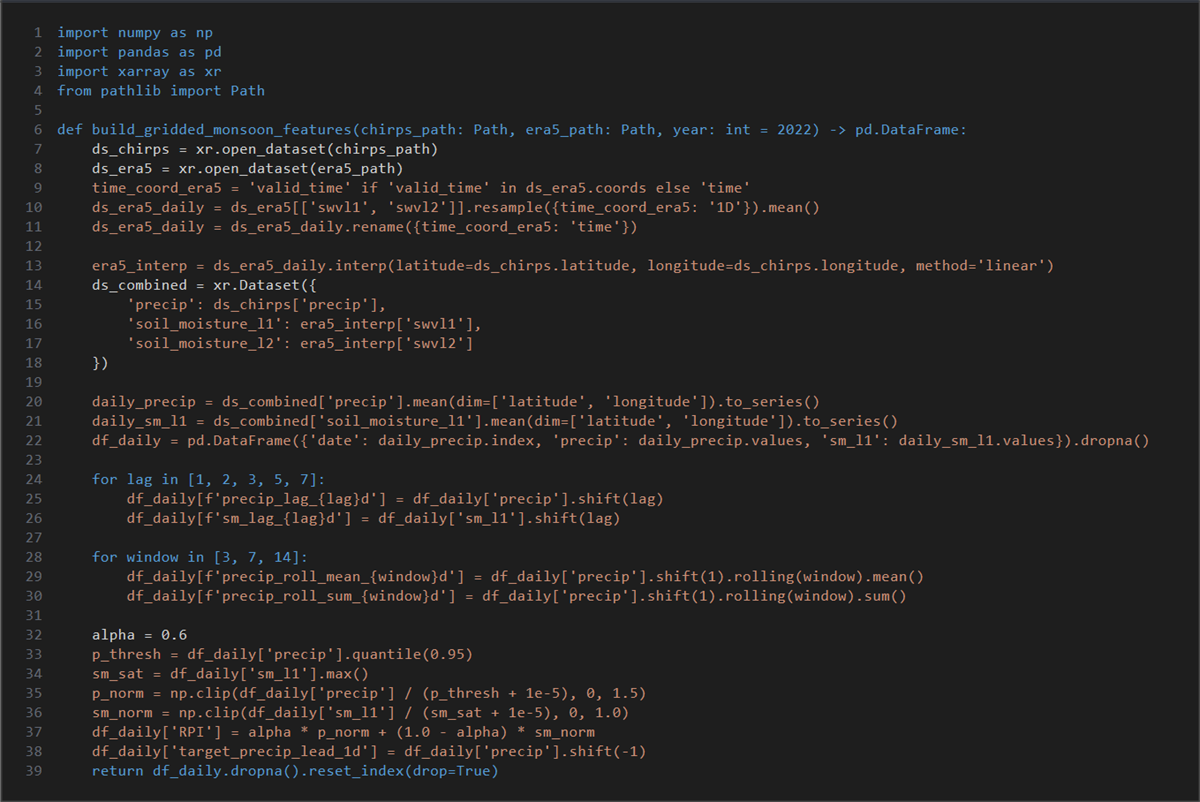
\includegraphics[width=\columnwidth]{snippet_features_rpi.png}
\caption{Feature engineering pipeline co-registering satellite precipitation with ERA5-Land soil moisture and computing the dynamic Runoff Potential Index.}
\label{fig:code_features_rpi}
\end{figure}

\begin{figure}[htbp]
\centering
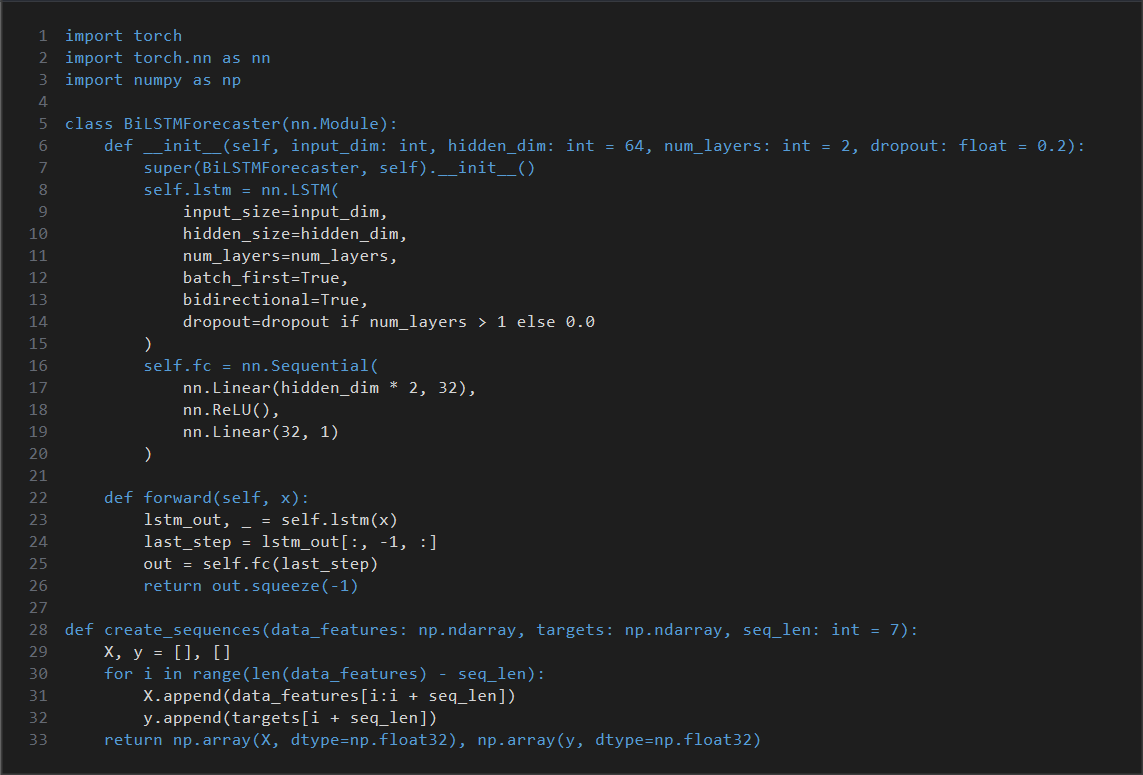
\includegraphics[width=\columnwidth]{snippet_bilstm_model.png}
\caption{PyTorch implementation of the 2-layer Bidirectional LSTM precipitation sequence forecaster with rolling lookback windowing.}
\label{fig:code_bilstm}
\end{figure}

\begin{figure}[htbp]
\centering
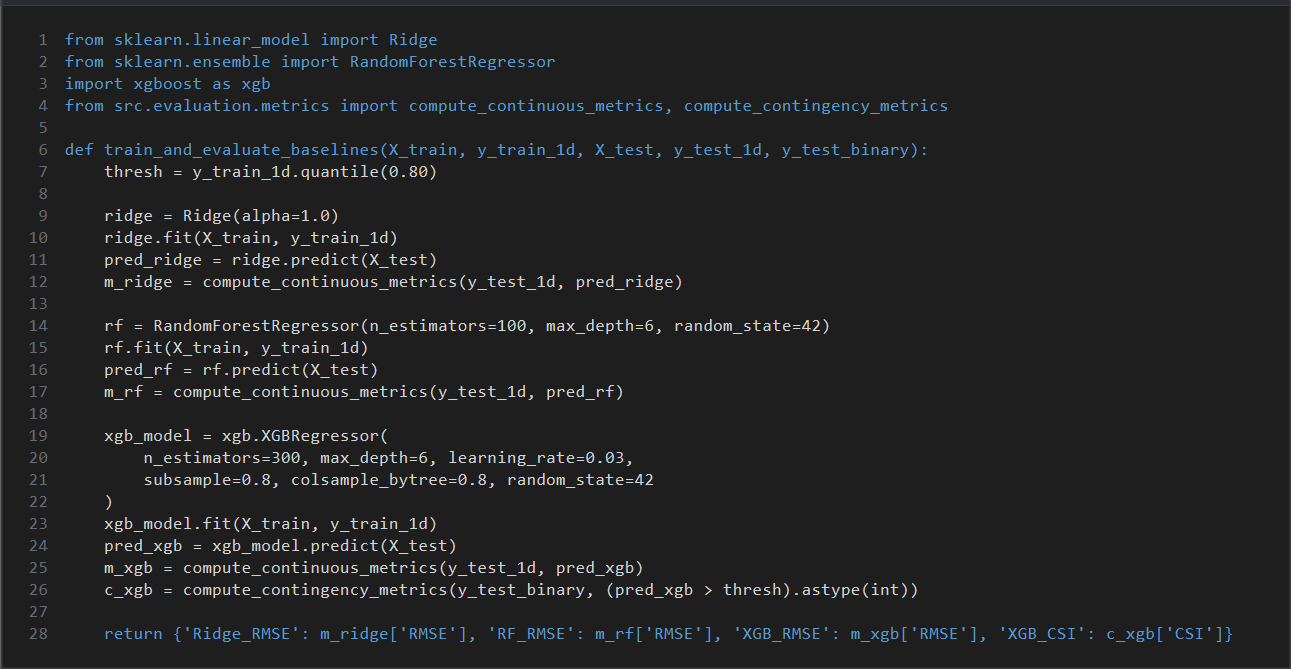
\includegraphics[width=\columnwidth]{snippet_baselines_xgb.png}
\caption{Baseline machine learning trainer and multi-horizon evaluation harness benchmarking Ridge, Random Forest, and tuned XGBoost models.}
\label{fig:code_baselines}
\end{figure}

\begin{figure}[htbp]
\centering
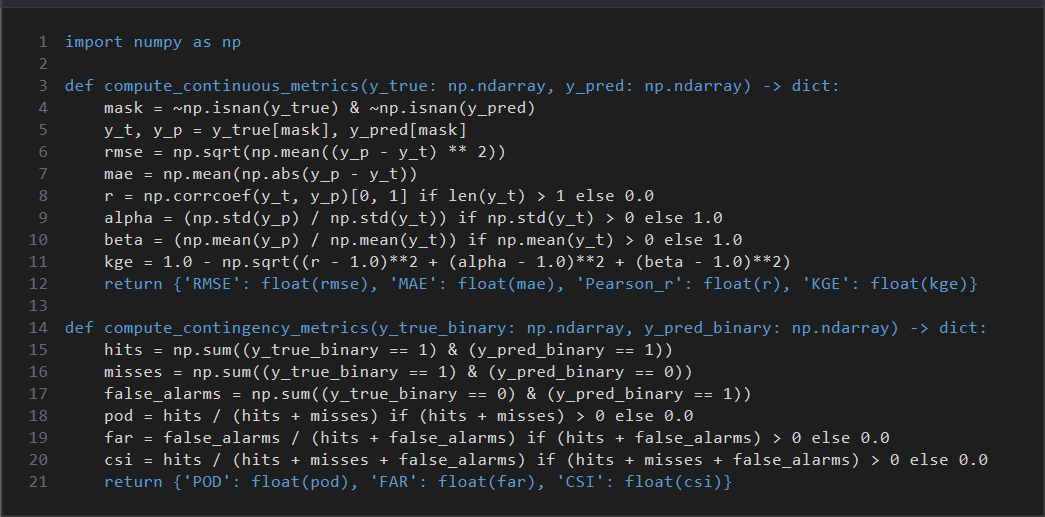
\includegraphics[width=\columnwidth]{snippet_evaluation_metrics.png}
\caption{Continuous hydrologic metric functions (RMSE, MAE, KGE) and contingency threshold evaluation metrics (POD, FAR, CSI).}
\label{fig:code_metrics}
\end{figure}

\end{document}
